\documentclass[14pt, hyperref={unicode}]{beamer}

% use the metropolis theme, with a black main color
\usetheme[titleformat = smallcaps]{metropolis}
\setbeamercolor{normal text}{fg=black, bg=white}

% add fade transition
\addtobeamertemplate{background canvas}{\transfade[duration=0.2]}{}

% set a frame footer to fit the purpose of the presentation
\setbeamertemplate{frame footer}{SOČ 2019}

% change frame footer and numbering color to gray to make it less intrusive
\setbeamercolor{frame footer}{fg=gray}
\setbeamercolor{frame numbering}{fg=gray}


% LANGUAGE %
%-========-%
\usepackage[czech]{babel} % czech language localization

% since appendix is only the last slide, change its name
\addto{\captionsczech}{\renewcommand*{\appendixname}{Děkuji za pozornost}}

% fixes the Czech/Slovak babel and booktabs packages clash
% https://tex.stackexchange.com/questions/111999/slovak-and-czech-babel-gives-problems-with-cmidrule-and-cline
\AtBeginDocument{\shorthandoff{-}}


% GRAPHICS %
%-========-%
\usepackage{graphicx}        % graphics package
\graphicspath{ {./images/} } % path to images

\usepackage{float} % floats in correct position (the [H] option)

\usepackage{subcaption} % for subfigures

\setlength{\fboxsep}{0pt}    % image border separation
\setlength{\fboxrule}{0.5pt} % image border thickness


% GRAPHS, CHARTS %
%-==============-%
\usepackage{pgf-pie} % pie charts

% define custom colors for the graph
\definecolor{azure}{RGB}{0,102,255}
\definecolor{red}{RGB}{255,0,0}

% change pie chart number separator from dot to comma
\usepackage{siunitx}
\sisetup{
  output-decimal-marker={,},
  group-separator={\,},
}
\def\ScanPercentage#1\afternumber{\SI{#1}{\percent}}

\usepackage{pgfplots} % bar charts


% CAPTIONS %
%-========-%
\usepackage[font=footnotesize,       % 10pt captions
            justification=centering, % center the captions
            figurename=Obr.,         % picture captions are "Obr."
            tablename=Tab.]{caption} % table captions are "Tab."


% TABLES          %
% requires: float %
%-===============-%
\usepackage{booktabs} % table formatting
\usepackage{multirow} % for creating multirow tables

% make each frame title appear in the bookmarks
% https://tex.stackexchange.com/questions/66519/make-each-frame-not-slide-appear-in-the-pdf-bookmarks-with-beamer
\usepackage{bookmark}
\usepackage{etoolbox}
\makeatletter
\apptocmd{\beamer@@frametitle}{\only<1>{\bookmark[page=\the\c@page,level=3]{#1}}}%
{\message{** patching of \string\beamer@@frametitle succeeded **}}%
{\message{** patching of \string\beamer@@frametitle failed **}}%
\makeatother


% MATH %
%-====-%
\usepackage{amsmath, amstext} % for typesetting math
\DeclareMathSymbol{.}{\mathord}{letters}{"3B} % change dot in math to a comma

% FONT AND ENCODING %
%-=================-%
\usepackage{fontawesome5} % use FontAwesome 5 for icons
\newfontfamily\mathfont{CMU Serif} % will be used for \LaTeX and \KaTeX commands
\usefonttheme[onlymath]{serif} % use a serif font for math


% LISTS %
%-=====-%
\setlength\leftmargini{0.4\leftmargini}
\setlength\leftmarginii{1.6\leftmargini}


% LOGOS, ICONS %
%-============-%
% KaTeX logo
\makeatletter
\DeclareRobustCommand{\KaTeX}{%
  K\kern -.19em
  {\sbox \z@ T\vbox to\ht \z@ {\hbox{%
  \check@mathfonts
  \fontsize\sf@size\z@
  \selectfont A}%
  \vss}%
}\kern -.15em
\TeX}
\makeatother


% OTHER %
%-=====-%
\usepackage{multido}

% browser icons
\newcommand{\Firefox}{\faIcon{firefox}}
\newcommand{\Chrome}{\faIcon{chrome}}
\newcommand{\IE}{\faIcon{internet-explorer}}
\newcommand{\Edge}{\faIcon{edge}}
\newcommand{\Safari}{\faIcon{safari}}
\newcommand{\Opera}{\faIcon{opera}}

% yes, no and N/A icons
\newcommand{\Yes}{\faIcon{check}}
\newcommand{\No}{\faIcon{times}}
\newcommand{\NA}{\faIcon{minus}}

% for making only certain icons monospaced
\NewDocumentCommand\fixfaIcon{ m s}{\makebox[1.5em][c]{\IfBooleanTF{#2}{\csname fa#1\endcsname*}{\csname fa#1\endcsname}}}

% for inserting appropriate icons to specific slide names
\newcommand{\Mobile}{\fixfaIcon{Mobile}*}
\newcommand{\Desktop}{\fixfaIcon{Desktop}}
\newcommand{\Book}{\fixfaIcon{Book}}

\newcommand{\Plus}{\fixfaIcon{Plus}}
\newcommand{\Minus}{\fixfaIcon{Minus}}

% ---------------------------------------------------------------------------- %

% title page settings
\title{\makebox[\linewidth]{Robotika jednoduše}}
\setbeamerfont{title}{size=\huge} % center the title

\date{\today}
\author{Tomáš Sláma}
\institute{Gymnázium Turnov}

\begin{document}
  \maketitle

  \begin{frame}{Motivace}
    \pause
    \begin{itemize}[<+->]
      \item vysoké uplatnění robotiky v dnešním světě
      \item nedostatek přístupných materiálů
      \item poskytnutí centralizovaného zdroje informací
    \end{itemize}
  \end{frame}

  \section{Technické provedení}

  \begin{frame}{Generování stránky}
    \pause
    \begin{itemize}[<+->]
      \item \textbf{Jekyll} -- generátor statických webů
      \item zdrojový kód z prostého textu
    \end{itemize}

    \vspace{\baselineskip}

    \begin{columns}[b, onlytextwidth]
      \setlength\topsep{0pt}
      \small
      \column<+->{0.5\textwidth}
        \begin{center}
          \large
          \Plus
        \end{center}
        \begin{itemize}[<+->]
          \itemsep0em
          \item vyšší bezpečnost
          \item jednoduché verzování
        \end{itemize}
      \column<+->{0.5\textwidth}
        \begin{center}
          \large
          \Minus
        \end{center}
        \begin{itemize}[<+->]
          \itemsep0em
          \item žádný dynamický obsah
          \item obtížnost nastavení
        \end{itemize}
    \end{columns}
  \end{frame}

  \begin{frame}{Automatizace provozu}
    \pause
    \begin{itemize}[<+->]
      \item \textbf{Python} -- skriptovací jazyk
      \begin{itemize}
        \item jednoduchá syntaxe
        \item rozsáhlá standardní knihovna
        \item vysoká míra abstrakce
      \end{itemize}
    \end{itemize}

    \begin{itemize}
      \item<+-> usnadnění provozu automatizováním
      \begin{itemize}[<+->]
        \item generování souboru sitemap.xml
        \item převodu do PDF
        \item komprimace obrázků
        \item minimalizace zdrojového kódu
        \item uploadu stránky přes FTP
      \end{itemize}
    \end{itemize}
  \end{frame}

  \section{Testování výkonu}

  \begin{frame}{Multiplatformnost}
    \pause
    \begin{minipage}[b]{\textwidth}
      \begin{table}[H]
        \caption{Funkčnost stránky na různých platformách}
        \scriptsize
        \centering
        \begin{tabular}{@{}rccccccccccccc@{}}
          \toprule
            & \multicolumn{6}{c}{Stolní počítač} & \phantom{abc} & \multicolumn{6}{c}{Mobilní zařízení} \\
          \cmidrule{2-7} \cmidrule{9-14}
            & \Firefox & \Chrome & \IE & \Edge & \Safari & \Opera && \Firefox & \Chrome & \IE & \Edge & \Safari & \Opera \\
          \midrule
            Obrázky     & \Yes & \Yes & \Yes & \Yes & \Yes & \Yes && \Yes & \Yes & \alert<4>{\NA} & \Yes & \Yes & \Yes \\
            Rovnice     & \Yes & \Yes & \Yes & \Yes & \Yes & \Yes && \Yes & \Yes & \alert<4>{\NA} & \Yes & \Yes & \Yes \\
            Vizualizace & \Yes & \Yes & \alert<3>{\No}  & \Yes & \Yes & \Yes && \Yes & \Yes & \alert<4>{\NA} & \Yes & \Yes & \Yes \\
            Formátování & \Yes & \Yes & \Yes & \Yes & \Yes & \Yes && \Yes & \Yes & \alert<4>{\NA} & \Yes & \Yes & \Yes \\
          \bottomrule
        \end{tabular}
      \end{table}
    \end{minipage}
  \end{frame}

  \begin{frame}{Doba načtení}
    \pause
    \begin{itemize}
      \item \textbf{WebPageTest} -- rychlost načtení stránky
    \end{itemize}

    \pause

    \begin{figure}[H]
      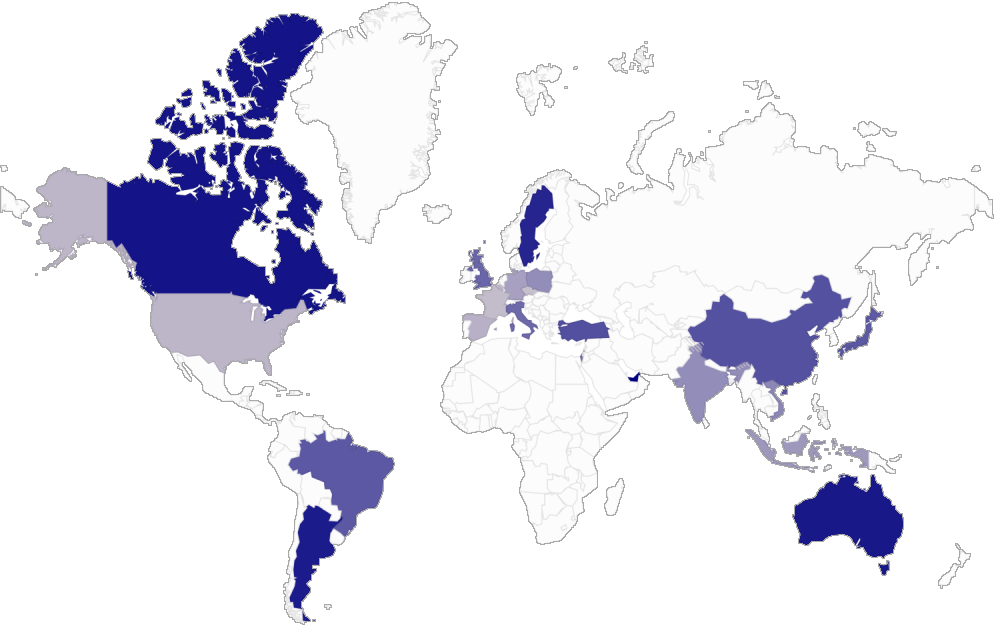
\includegraphics[width=\textwidth,height=0.6\textheight,keepaspectratio]{map.png}
      \caption{Mapa dob načtení stránky (od \alert<4>{\SI{1.356}{\second}} do \alert<5>{\SI{4.215}{\second}})}
    \end{figure}
  \end{frame}

  \section{Tvorba obsahu}

  \begin{frame}[fragile]{Renderování rovnic}
    \pause
    \begin{itemize}[<+->]
      \item {\mathfont\textbf{\KaTeX}} -- JavaScriptová knihovna
      \item renderování rovnic z {\mathfont\LaTeX}ové notace
    \end{itemize}

    \onslide<+->
    \begin{equation}
      \small
      \verb|$$\sum_{i=1}^{n}i=\frac{n(n+1)}{2}$$|
    \end{equation}

    \onslide<+->
    \begin{equation}
      \small
      \sum_{i=1}^{n} i = \frac{n(n+1)}{2}
    \end{equation}
  \end{frame}

  \begin{frame}[fragile]{Tvorba ilustrací}
    \pause
    \begin{itemize}
      \item \textbf{InkScape} -- vektorová grafika
    \end{itemize}

    \pause

    \begin{figure}[H]
      \centering

      \subcaptionbox{Pohyb robota po kružnici}{\fbox{
\includegraphics[width=.3\linewidth]{illustration1.png}}}%
      \hfill
      \subcaptionbox{Odhad pozice pohybem po přímce}{\fbox{
\includegraphics[width=.3\linewidth]{illustration2.png}}}%
      \hfill
      \subcaptionbox{Odhad pozice pohybem po kružnici}{\fbox{
\includegraphics[width=.3\linewidth]{illustration3.png}}}%

      \caption{Příklad ilustrací článků}
    \end{figure}
  \end{frame}

  \begin{frame}[fragile]{Ověření správnosti kódu}
    \pause
    \begin{itemize}
      \item \textbf{VEX EDR} -- robotická stavebnice
      \begin{itemize}
        \item programování v jazyce Python
      \end{itemize}
    \end{itemize}

    \pause

    \begin{figure}[H]
      \centering

      \subcaptionbox{Boční pohled na model robota}{\fbox{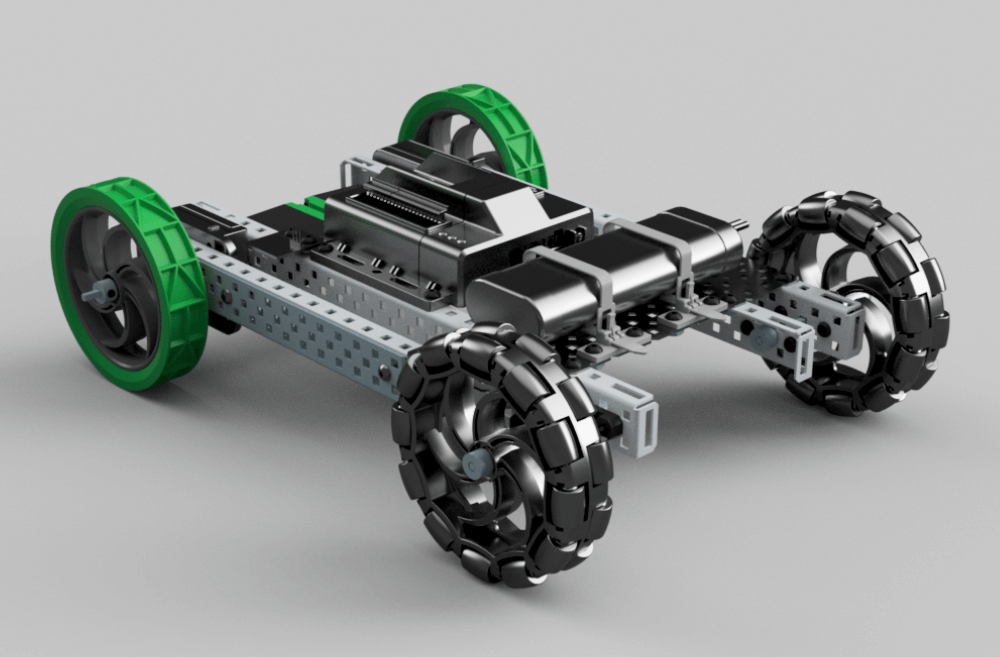
\includegraphics[width=.475\linewidth]{robot1.png}}}%
      \hfill
      \subcaptionbox{Vrchní pohled na model robota}{\fbox{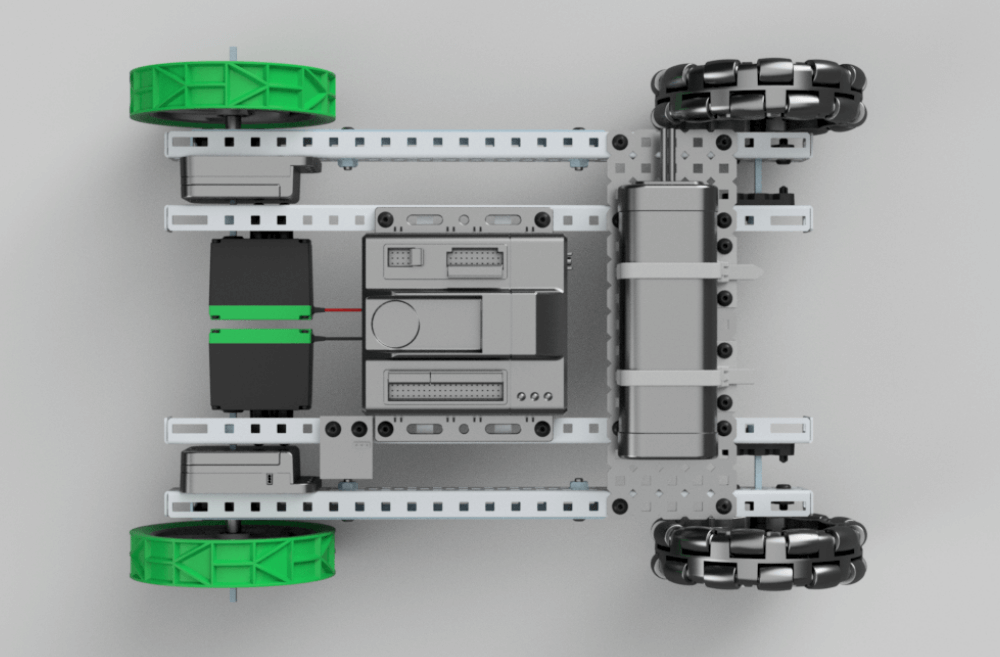
\includegraphics[width=.475\linewidth]{robot2.png}}}%

      \caption{3D model robota, vytvořen v CAD programu Fusion 360}%
    \end{figure}
  \end{frame}

  \section{Režimy prohlížení}

  \begin{frame}{\texorpdfstring{Plný vzhled\hfill\Desktop}{Plný vzhled}}
    \pause
    \begin{figure}[H]
      \fbox{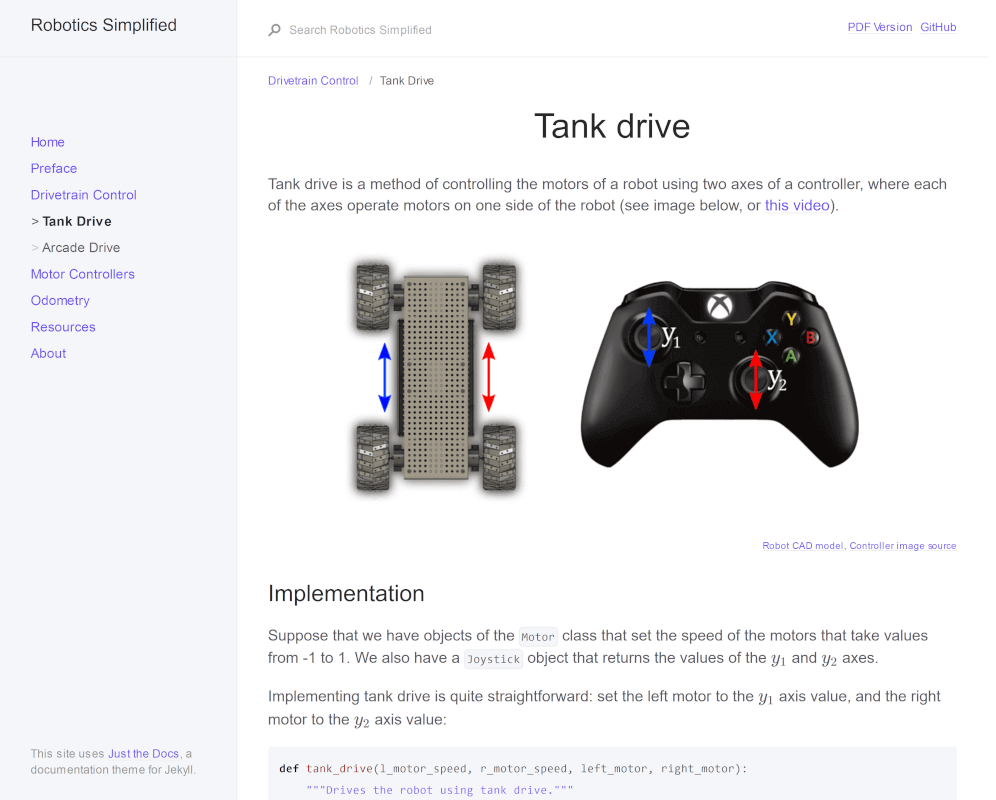
\includegraphics[width=\textwidth,height=0.7\textheight,keepaspectratio]{full-version.png}}
      \caption{Plný vzhled webové stránky}
    \end{figure}
  \end{frame}

  \begin{frame}{\texorpdfstring{Kompaktní vzhled\hfill\Mobile}{Kompaktní vzhled}}
    \pause
    \begin{figure}[H]
      \centering

      \subcaptionbox{Stránka bez menu}{\fbox{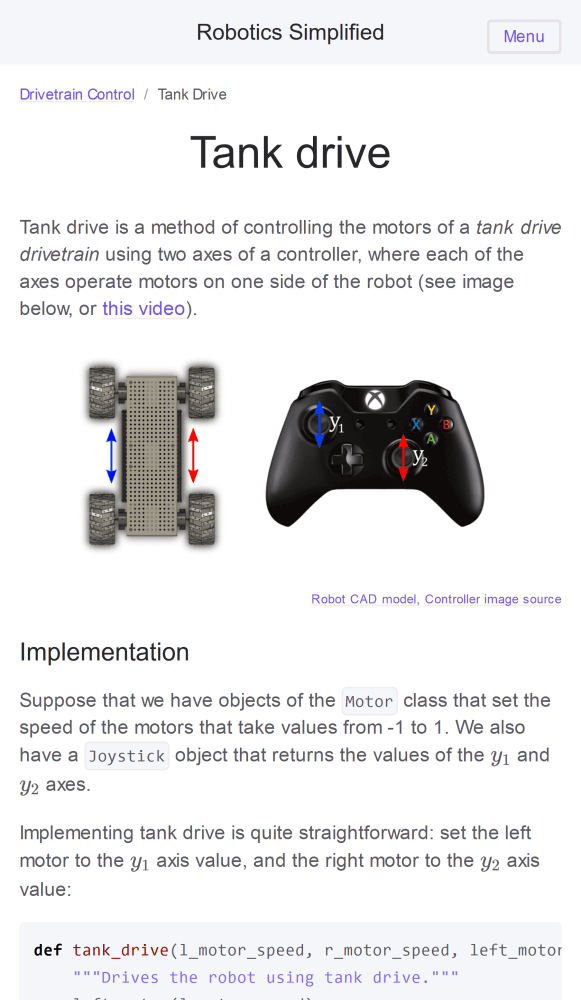
\includegraphics[width=\textwidth,height=0.6\textheight,keepaspectratio]{compact-version-1.png}}}%
      \qquad
      \subcaptionbox{Stránka s menu}{\fbox{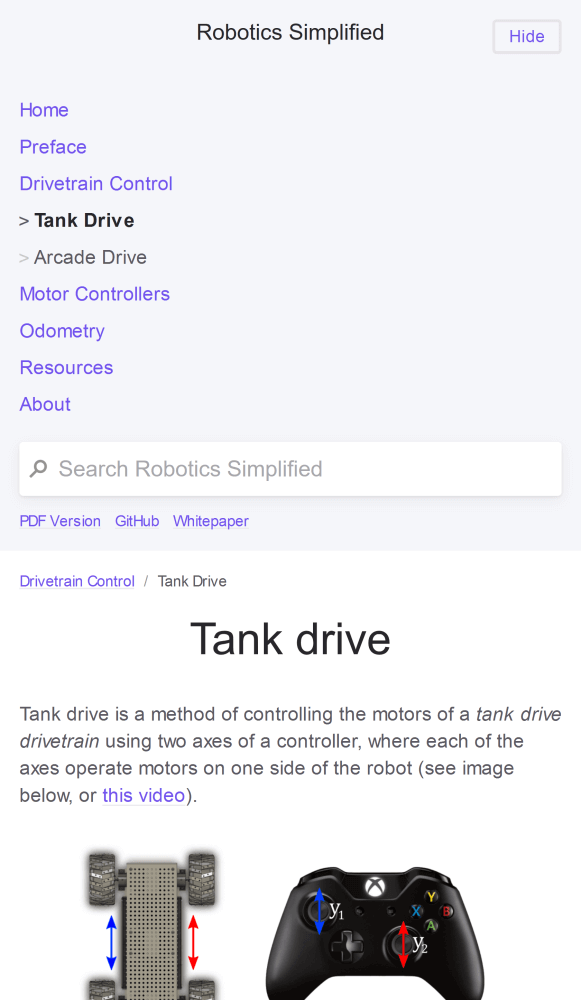
\includegraphics[width=\textwidth,height=0.6\textheight,keepaspectratio]{compact-version-2.png}}}%

      \caption{Kompaktní vzhled webové stránky}%
    \end{figure}
  \end{frame}

  \begin{frame}{\texorpdfstring{PDF verze\hfill\Book}{PDF verze}}
    \pause
    \begin{figure}[H]
      \fbox{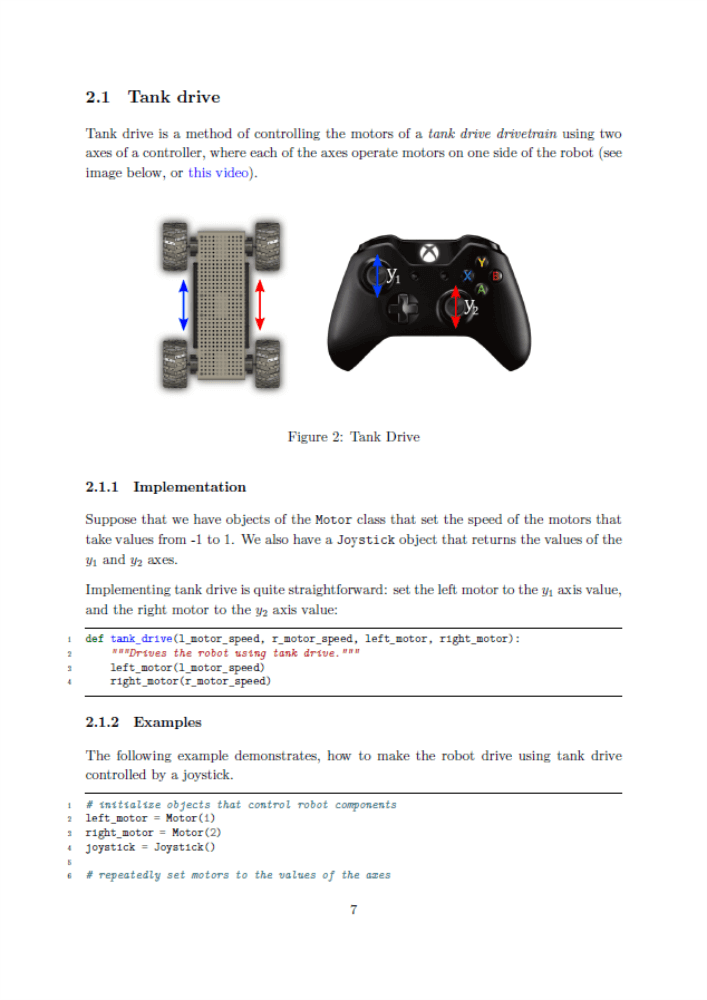
\includegraphics[width=\textwidth,height=0.7\textheight,keepaspectratio]{pdf-version.png}}
      \caption{PDF verze webové stránky}
    \end{figure}
  \end{frame}

  \section{Návštěvnost}

    \begin{frame}{Sbírání dat}
      \pause
      \begin{itemize}[<+->]
        \item \textbf{Google Analytics} -- data návštěvníků a jejich interakce se stránkou
        \begin{itemize}
          \item věk, pohlaví, lokace
          \item zařízení, prohlížeč
          \item délka návštěvy
        \end{itemize}
      \end{itemize}

      \begin{itemize}[<+->]
        \item \textbf{Google Search Console} -- Google vyhledávání
        \begin{itemize}
          \item statistiky o pozici na Googlu
        \end{itemize}
      \end{itemize}
    \end{frame}

  \begin{frame}{Pohlaví a věk}
      \pause
      \begin{figure}
        \begin{minipage}[b]{0.5\textwidth}
          \multido{\n=2+1}{3}{
            \only<\ifnum\n<3 {-2}\else \ifnum\n=3 {3} \else {4-} \fi \fi>{
              \scriptsize
              \centering
              \begin{tikzpicture}[scale=0.64]
                \pie[color={\ifnum\n=3 mLightBrown\else azure\fi, red}, rotate=-35, before number=\ScanPercentage, after  number ={ }\%,]{91.2/Muži, 8.8/Ženy}
              \end{tikzpicture}
              \captionof{figure}{Pohlaví návštěvníků}
              \label{img:Pohlaví návštěvníků}
            }
          }
        \end{minipage}\hfill
        \begin{minipage}[b]{0.5\textwidth}
          \multido{\n=3+1}{2}{
            \only<\ifnum\n<4 {-3}\else {4-}\fi>{
              \scriptsize
              \centering
              \begin{tikzpicture}
                \begin{axis}[
                  symbolic x coords={18--24,,25--34,,35--44,,45--54},
                  xtick={18--24,25--34,35--44,45--54},
                  ylabel={Procento návštěvníků},
                  xlabel={Věková kategorie (let)},
                  bar width=0.5cm,
            width=\textwidth,
                  enlarge x limits=0.18,
                  ymin=0, ymax=60,
                  nodes near coords={\pgfmathprintnumber\pgfplotspointmeta{ }\%},
                  yticklabel={\pgfmathparse{\tick}\pgfmathprintnumber{\pgfmathresult}{ }\%}]
                  \addplot[ybar,fill=azure] coordinates {(18--24, 18.9)};
                  \addplot[ybar,fill={\ifnum\n=4 mLightBrown\else azure\fi}] coordinates {(25--34, 48.4)};
                  \addplot[ybar,fill=azure] coordinates {(35--44, 18.0)};
                  \addplot[ybar,fill=azure] coordinates {(45--54, 14.7)};
                \end{axis}
              \end{tikzpicture}
              \captionof{figure}{Věk návštěvníků}
              \label{img:Věk návštěvníků}
            }
          }
        \end{minipage}
      \end{figure}
    \end{frame}

  \begin{frame}{Prohlížeč a lokace}
      \pause
    \begin{figure}
      \begin{minipage}[b]{0.5\textwidth}
        \begin{table}[H]
          \caption{Lokace návštěvníků}
          \scriptsize
          \centering
          \begin{tabular}{lr}
              \toprule
                \emph{Země} & \emph{Návštěvníci} \\
              \midrule
                \alert<3>{Spojené státy} & \alert<3>{\num{240}} \\
                Česká republika & \num{35} \\
                \alert<3>{Spojené království} & \alert<3>{\num{20}} \\
                \alert<3>{Kanada} & \alert<3>{\num{17}} \\
                Německo & \num{10} \\
                Japonsko & \num{10} \\
                Čína & \num{8} \\
                Indie & \num{8} \\
                Španělsko & \num{7} \\
                Nizozemí & \num{7} \\
              \bottomrule
            \end{tabular}
          \end{table}
      \end{minipage}\hfill
      \begin{minipage}[b]{0.5\textwidth}
        \begin{table}[H]
          \caption{Prohlížeč návštěvníků}
          \scriptsize
          \centering
          \begin{tabular}{lr}
              \toprule
                \emph{Prohlížeč} & \emph{Návštěvníci} \\
              \midrule
                \alert<4>{Chrome} & \alert<4>{\num{226}} \\
                \alert<5>{Firefox} & \alert<5>{\num{111}} \\
                Safari & \num{85} \\
                Android Webview & \num{14} \\
                Internet Explorer & \num{6} \\
                Opera & \num{6} \\
                Edge & \num{5} \\
                Samsung Internet & \num{5} \\
                Neurčeno & \num{4} \\
                Cốc Cốc & \num{1} \\
              \bottomrule
            \end{tabular}
          \end{table}
        \end{minipage}
      \end{figure}
    \end{frame}

  \appendix

  {\setbeamertemplate{frame footer}{}
  \begin{frame}[standout]
    Děkuji za pozornost
  \end{frame}}
\end{document}
